\documentclass{llncs}

\usepackage{amsmath} % for equation*
\usepackage{color}
\usepackage{hyperref}
\usepackage{graphicx}
\definecolor{darkgreen}{rgb}{0,0.7,0}

% Fix link colors
\hypersetup{
    colorlinks = true,
    linkcolor=red,
    citecolor=red,
    urlcolor=blue,
    linktocpage % so that page numbers are clickable in toc
}

\newcounter{ques}
\setcounter{ques}{1}

\newcommand{\quest}[2]{\paragraph{}\textbf{Q\theques} - #1\stepcounter{ques} }

\newcommand{\answer}[1]{
\noindent\color{red}A: #1\color{black}}
\title{COMP 445 -- Theoretical Assignment 3 (TA3)}

\author{Tristan Glatard\\
  \href{mailto:tristan.glatard@concordia.ca}{tristan.glatard@concordia.ca}\\
  \vspace*{0.3cm}
  }

\institute{Concordia University\\
  Department of Computer Science and Software Engineering}

\begin{document}

\maketitle

All questions will receive equal points. Please submit your assignment
as a pdf file on Moodle. The name of the pdf file must contain your
name and student id. Your name and student id must also appear in the
header of the pdf document. Please answer the questions in the order
used below and indicate the question number before your answer (e.g.,
\textbf{Q1}). Wherever possible, briefly indicate the method used to
obtain a numerical value, e.g., mathematical formula. Due date:
\textbf{April 7, 11:55pm}.

  \setlength{\tabcolsep}{12pt}

\section{Network Layer}

\quest{Briefly describe the two main functions of the network layer, namely forwarding and routing.}

\answer{See slide 5. Forwarding moves packets from router's input to
  appropriate router output. Routing determines route taken by packets
  from source to destination.}

\quest{Explain the primary role of the \texttt{identification} field in the IPv4 datagram format.}

\answer{See slide 34. This field is used for fragmentation and
  reassembly.}

\quest{Consider two hosts A and B located in a NAT'ed network. Assume
  that the IP addresses of A and B are 10.0.0.1 and 10.0.0.2,
  respectively. Assume that the IP addresses of the NAT router are
  10.0.0.3 (LAN side) and 132.205.244.42 (WAN side). What will be the
  content of the NAT translation table after A and B connected to the
  Web server at \texttt{www.concordia.ca} (132.205.244.70)? Assume
  that A connected from port 1234 and that B connected from port
  1235.}

\answer{See slide 58. Assuming that the router uses ports 2345 and 2346, the NAT table entries would be:\\
  \begin{tabular}{cc}
    WAN side              & LAN side \\
    \hline
    132.205.244.42, 2345  & 10.0.0.1, 1234 \\
    132.205.244.42, 2346  & 10.0.0.2, 1235 \\
  \end{tabular}
}

\newpage
\quest{The content between the two lines below was captured using
  Wireshark:
  
\noindent \hrulefill\\
\begin{small}
  \textbf{Type: 8} (Echo (ping) request)\\
  Code: 0\\
  Checksum: 0x068c [correct]\\
  Checksum Status: Good\\
  Identifier (BE): 4737 (0x1281)\\
  Identifier (LE): 33042 (0x8112)\\
  Sequence number (BE): 1 (0x0001)\\
  Sequence number (LE): 256 (0x0100)\\
  Response frame: 2\\
  Timestamp from icmp data: Mar 20, 2017 10:58:19.000000000 EDT\\
  Timestamp from icmp data (relative): 0.514140297 seconds\\
\vspace*{-0.3cm}
\hrulefill\\
\end{small}
\begin{enumerate}
\item To which protocol does this content correspond to?
\item To which layer in the Internet model does this protocol belong to?
\item What is the meaning of the string in bold face (\textbf{Type 8})? 
\item Describe a possible follow-up message for this content, i.e.,
  how a host may respond to this message. Only a
  high-level description of the message is expected, i.e., you don't
  have to write the complete message explicitly.
\end{enumerate}
}

\answer{
  \begin{enumerate}
  \item ICMP
  \item Network layer
  \item Echo request
  \item Echo reply
  \end{enumerate}
}

\quest{\underline{Using the Dijkstra algorithm}, compute the least-cost
  paths from A to all the other nodes in the graph below. Your answer
  will have to detail the successive iterations of the algorithm.}


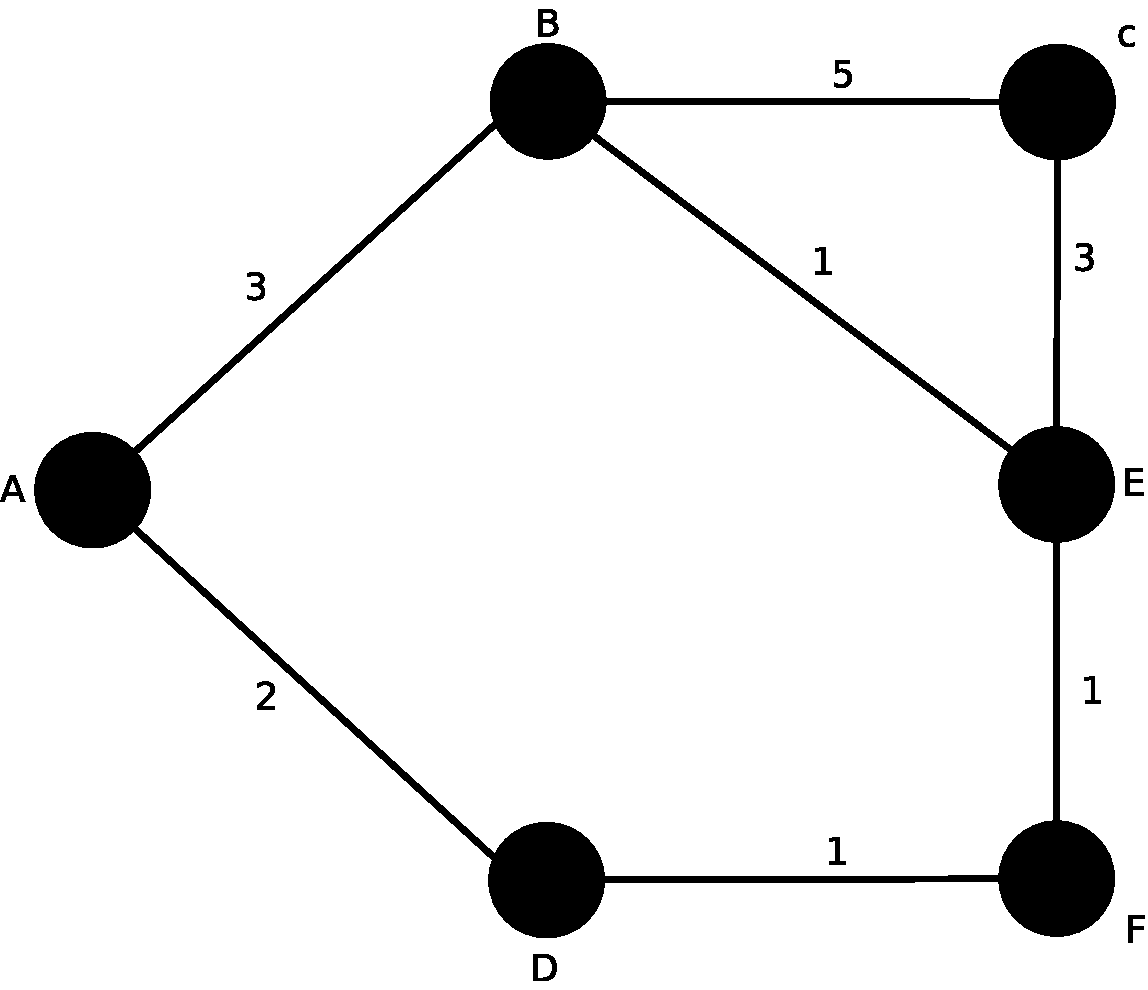
\includegraphics[width=0.5\textwidth]{graph.pdf}

\answer{
  The following table uses the notations on slides 79-80 of the lecture on the Network Layer.\\
  \begin{tabular}{lcccccc}
    N'     & B   & C        & D   & E        & F        & G\\
    A      & \underline{1,A} & $\infty$ & 4,A & $\infty$ & $\infty$ & $\infty$ \\
    AB     &     & \underline{2,B}      & 4,A & 5,B      & 4,B      & $\infty$ \\
    ABC    &     &          & \underline{3,C} & 5,B      & 4,B      & $\infty$ \\
    ABCD   &     &          &     & \underline{4,D}      & 4,B      & 4,D \\
    ABCDE  &     &          &     &          & \underline{4,B}      & 4,D      \\
    ABCDEF &     &          &     &          &          & \underline{4,D}      \\
    ABCDEFG&     &          &     &          &          &          \\
  \end{tabular}
}

\quest{Routing Information Protocol (RIP). Starting from the initial
  RIP table in C shown below, suppose that C receives from A the following
  advertisement. Will the table in C change? If so how?
  \begin{itemize}
\item  Original RIP table in C:\\
\begin{tabular}{ccc}
  Destination subnet & Next router & Hops to destination \\
  \hline
  u & - & 1\\
  v & D & 3\\
  w & D & 4 \\
  x & A & 3\\
\end{tabular}
\item \vspace*{1cm}Advertisement received by C from A:\\
\begin{tabular}{ccc}
  Destination subnet & Next router  & Hops to destination\\
  \hline
  u & C & 2\\
  v & B & 2\\
  w & - & 1 \\
  x & B & 2\\
\end{tabular}
\end{itemize}
}

\answer{New table in C:\\
  \begin{tabular}{ccc}
    Destination subnet & Next router & Hops to destination \\
    \hline
    u & - & 1\\
    v & D & 3\\
    w & \textbf{A} & \textbf{2} \\
    x & A & 3\\
  \end{tabular}
}


\section{Link Layer}

\quest{(P2 in Textbook, 6th edition). Give an example showing that
  two-dimensional parity checks can correct and detect a single bit
  error. Show a double-bit error that can be detected but not
  corrected.}

\answer{See slide 12.}

\quest{(R6 in Textbook, 6th edition). In CSMA/CD, after the fifth collision, what is the
  probability that a node chooses K=4? The result K=4 corresponds to a
  delay of how many seconds on a 10 Mbps Ethernet?}

\answer{See slide 33. After the fifth collision, K will be chosen at
  random in \{0,2$^5$-1\}, that is, in \{0,31\}. The probability to
  choose K=4 is therefore $\frac{1}{32}$. The corresponding delay is
  $\frac{4 \times 512}{10.10^6}=2.10^{-4}$s.}

\quest{What is the MAC address used for broadcast? Explain when and
  why such a broadcast address is used in ARP (Address Resolution
  Protocol).}

\answer{See slide 46. Broadcast address: FF:FF:FF:FF:FF:FF. This
  address is used to broadcast ARP queries. ARP queries cannot be
  directed to a specific host since only a host knows its MAC address
  and the purpose of the ARP query is precisely to ask for this MAC
  address.}

\quest{What is the main difference between Pure Aloha and Slotted Aloha? Are there any
circumstances where Pure Aloha would perform better than Slotted Aloha? If so, give
such circumstances/conditions. If no, explain why Pure Aloha could never perform better
that Slotted Aloha.}

\answer{See slides 24-28. The main difference between pure and slotted
  Aloha is that slotted Aloha requires frames to be transmitted in
  specific slots while this is not the case for pure Aloha. As
  detailed in the slides, the maximal efficiency for pure Aloha is
  half of slotted Aloha's, which suggests that slotted Aloha performs
  much better than pure Aloha (accepted answer). However, in practice,
  there are situations where pure Aloha's efficiency might become
  higher than slotted Aloha's. For instance, if there is only a single
  transmitting host, and if this host is sending very small frames,
  then most of the slots will be wasted in slotted Aloha while the
  channel will be continuously used in pure Aloha. It should be noted
  that this situation violates the assumptions in slide 24 though.  }

\end{document}
